\section{Results and Discussion}\label{sec:architecture}

Approbation of the developed web-application on real data was carried out. Several brands from one category were chosen for their handling by the service. The number of references of each brand in "interviewed" users tweets was returned at the exit. Thus, this service makes the comparative analysis of brands popularity in the microblog that corresponds to a state of affairs in a real life.

Also operation performance of application was checked. The different number of the analyzed accounts was entered. The maximum number of users, whose tweets were used, was 500 until the program fell. It's not enough for such a service. But the number of successfully processed information sharply increases after deployment the service in the cloud infrastructures.


The request lifecycle of the developed application is presented on the picture \ref {fig:requestLifecycle}.

\begin{figure}[tbh]
\centering
\caption{The request lifecycle of the developed application}
\label{fig:requestLifecycle}
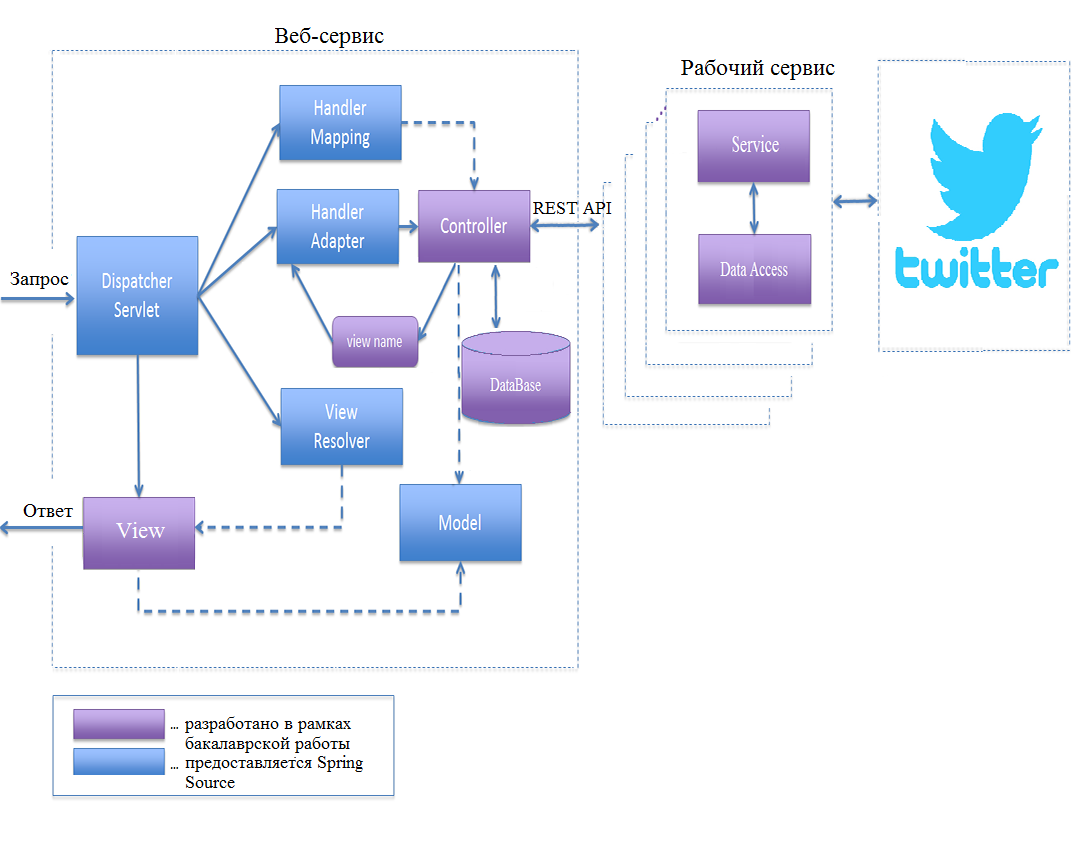
\includegraphics[width=\linewidth]{requestLifecycle}
\end{figure}